 \documentclass{article}
\usepackage[utf8]{inputenc}
\usepackage[top=3cm, bottom=3cm, left=3cm,right=3cm]{geometry}
%\usepackage[numbers,round]{natbib}
\usepackage{natbib}
\setcitestyle{aysep={}} 
\usepackage{graphicx}
\usepackage{color}
\usepackage{amsmath}
\usepackage{setspace}
\usepackage{amsmath}
\usepackage{mathtools}
\usepackage{bbm}
\usepackage{float}
\usepackage{hyperref}
\usepackage[super]{nth}

\parindent0cm
\parskip0.5cm
\hyphenpenalty=10000
\pretolerance=10000
\usepackage{lineno}
\linenumbers

\makeatletter
\newcommand{\customlabel}[2]{
\protected@write \@auxout {}{\string \newlabel {#1}{{#2}{}}}}
\makeatother

\renewcommand\footnote[2][]{\relax}

\begin{document}
{\Large Validation of dated phylogenies in microbial population genetics}


\vspace*{2cm}
Xavier Didelot$^{1,*}$, Paolo Ribeca$^{2,3}$, ...

\vspace*{2cm}
$^1$ School of Life Sciences and Department of Statistics, University of Warwick, United Kingdom\\\\
$^2$ UK Health Security Agency, London, United Kingdom\\\\
$^3$ Biomathematics and Statistics Scotland, The James Hutton Institute, Edinburgh, United Kingdom\\\\
$^*$ Corresponding author. Tel: 0044 (0)2476 572827. Email: \verb+xavier.didelot@gmail.com+

%\newpage
%\section*{ABSTRACT}
%TODO

\newpage
\section*{INTRODUCTION}

Dated phylogenies, also known as tip-calibrated, time-stamped or time-calibrated phylogenies, have become a ubiquitous tool in the study of microbial population genetics 
\citep{Drummond2003,Biek2015,rieuxInferencesTipcalibratedPhylogenies2016}. In a dated phylogeny, the branch lengths are measured in a unit of time, for example years or days,
rather than a unit of evolution as in a standard phylogeny. Consequently, the tips of a dated phylogeny are aligned with the (typically known) dates of sampled genomes and
the internal nodes are aligned with the (typically inferred) dates of common ancestors between the genomes.
Many tools exist to build dated phylogenies, either from a sequence alignment using for example BEAST \citep{Suchard2018} or BEAST2 \citep{Bouckaert2019}, or by
dating the nodes of a standard phylogeny, using for example 
LSD \citep{To2016}, node.dating \citep{Jones2017}, treedater \citep{Volz2017}, BactDating \citep{Didelot2018} and TreeTime \citep{Sagulenko2018}.
The dated phylogeny is interesting in itself since it depicts the ancestral relationships of sampled genomes
over time, but it is also often used as the foundation for further analysis \citep{Didelot2022}, such as inference
of demographics \citep{Baele2016}, phylogeography \citep{Lemey2009} 
or transmission between hosts \citep{Didelot2017}.

There are many factors that can invalidate the results of a dated phylogenetics analysis.
This includes in particular the confounding effect that population structure can have on dating 
\citep{Duchene2015a,Murray2016}. This is especially true when the substructures are 
imbalanced \citep{ducheneTreeImbalanceCauses2015}, are sampled
at different dates \citep{tongComparisonMethodsEstimating2018}, have different clock rates
\citep{wertheimInconsistenciesEstimatingAge2012}  and when the population structure is strong 
\citep{navascuesElevatedSubstitutionRate2009}. 
More generally, any incorrect assumptions made by the model under which the dating analysis is performed
can invalidate the results.

One approach that has been used to ensure that there are no incorrect assumptions being made in the 
model is to perform inference under multiple models and perform model comparison,
typically by computing a Bayes Factor \citep{Baele2012,Li2012,bouckaertBModelTestBayesianPhylogenetic2017}. 
However, this requires multiple runs under different models, and only provides a relative measure
of model appropriateness, with no indication of how good the best model actually is in absolute terms.
Another related line of research involves testing the significance of the temporal signal 
\citep{Duchene2015a,Duchene2020}. This can be done for example by 
comparing results with and without dates \citep{Rambaut2000} or by 
randomizing the leaf dates \citep{Duchene2015a}. 

Here we present an alternative approach, in which we seek to evaluate
the correctness of an inference and detect if there are any reasons to believe that the inference is not valid.
This approach is sometimes referred to as model checking, model diagnostics or model validation, 
and it is complementary with the model comparison methodology mentioned above. 
We study the distribution of residuals after fitting a model, following methodology
reminiscent of regression models
\citep{coxGeneralDefinitionResiduals1968,dunnRandomizedQuantileResiduals1996},
but also previously applied more generally for example to
epidemic models \citep{lauNewModelDiagnostics2014} or 
 Hidden Markov Models \citep{zucchini2009hidden,buckbyModelCheckingHidden2020}.

We use simulated datasets to demonstrate that this approach can detect a wide range of problems
in the inference, including the aforementioned confounding effect of population structure
\citep{Murray2016}. 
We also demonstrate the usefulness of this approach in practice on real datasets.

\section*{RESULTS}

\subsection*{General approach}

\begin{figure}[t!]
\begin{center}
A\hspace*{6cm}B\hspace*{6cm}~\\
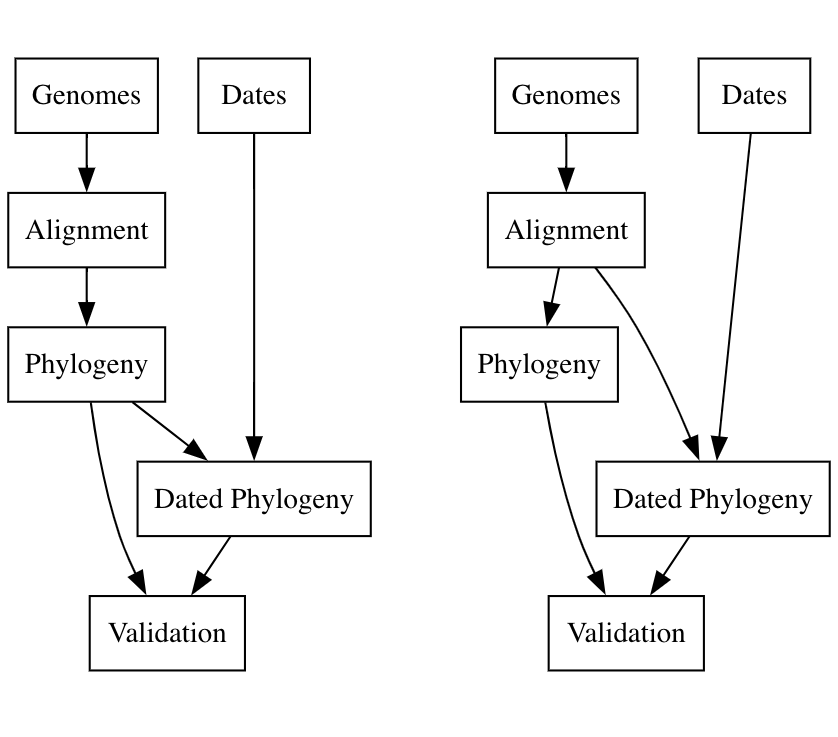
\includegraphics[width=10cm]{fig1.png}
\end{center}
\caption{(A) General approach for validation of a dated phylogeny built by dating the nodes of a standard phylogeny. (B) General approach for validation of a dated phylogeny built directly from a sequence alignment.
\label{fig:approach}}
\end{figure}

We want to validate a dated phylogeny $\mathcal{D}$, previously constructed using
any method. We propose to do so by comparing the dated phylogeny $\mathcal{D}$ with 
an undated phylogeny $\mathcal{L}$. 
If the method used to construct $\mathcal{D}$ involved dating the nodes of an undated
phylogeny, for example TreeTime \citep{Sagulenko2018} or treedater \citep{Volz2017}, 
then this is readily available for validation and we therefore focus on this case in this article
(Figure \ref{fig:approach}A). However, the validation methodology
below can also be applied to methods that build a dated phylogeny directly from the alignment
such as BEAST \citep{Suchard2018},
simply by constructing a separate undated phylogeny from the same alignment using
for example PhyML \citep{Guindon2010} or RAxML \citep{Stamatakis2015} 
(Figure \ref{fig:approach}B). For each branch in the dated phylogeny $\mathcal{D}$ we can
consider its inferred length, the number of substitutions happening on that branch in the standard phylogeny
$\mathcal{L}$, and the model and parameters used when building the dated phylogeny $\mathcal{D}$,
in order to compute a residual for that branch (see Methods). If the inference is valid,
these residuals will follow their theoretical distribution
\citep{coxGeneralDefinitionResiduals1968,dunnRandomizedQuantileResiduals1996}. 
We use this property as a way to test the validity of the dated phylogeny $\mathcal{D}$.

\subsection*{Motivating example}

\begin{figure}[p!]
\begin{center}
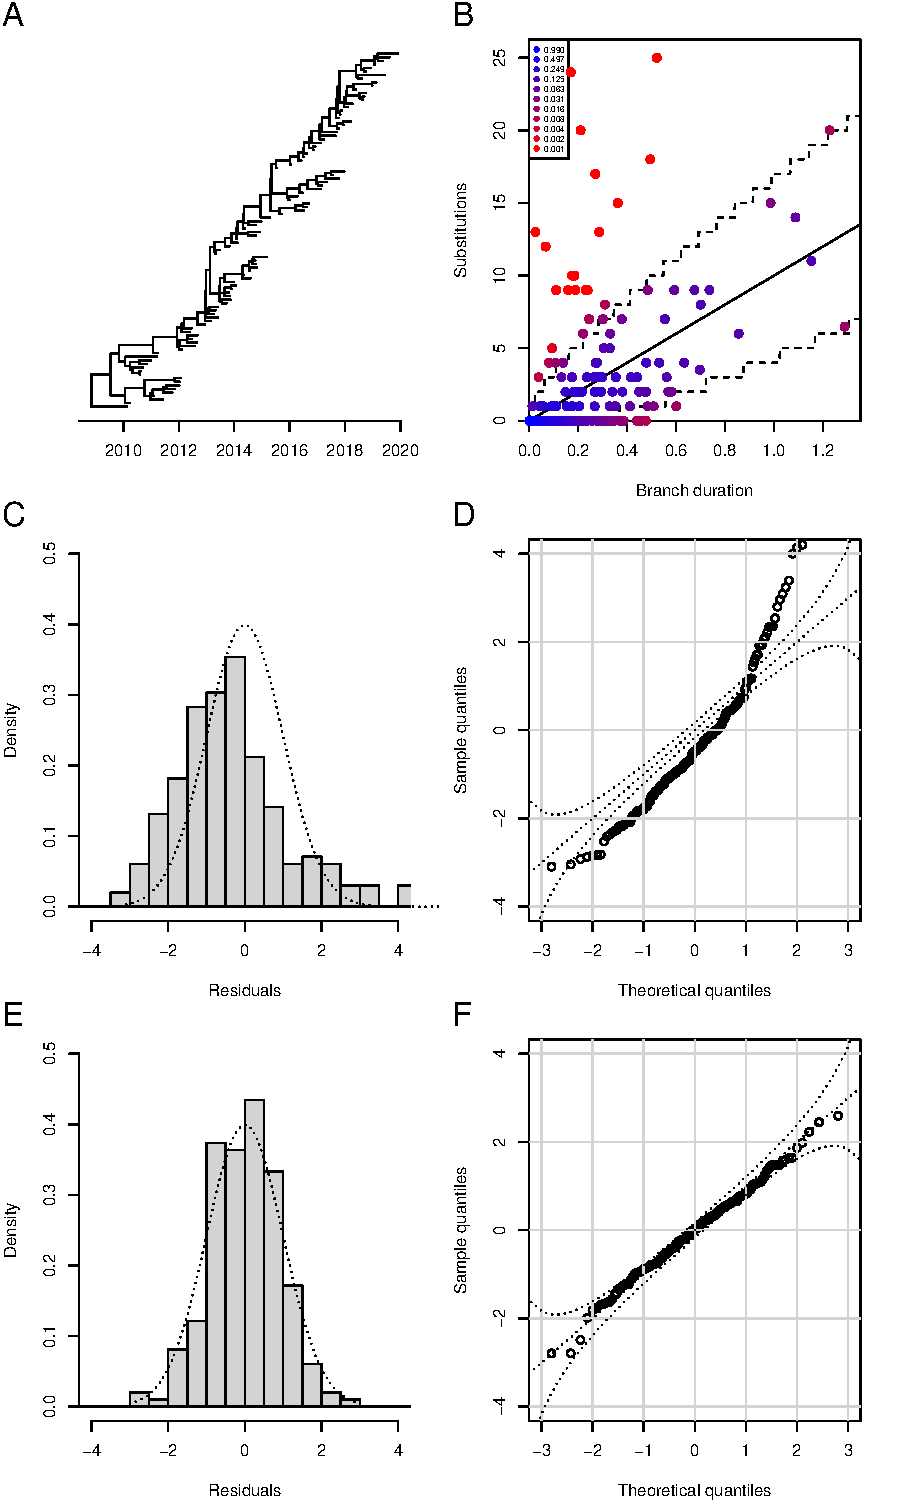
\includegraphics[width=10cm]{example.pdf}
\end{center}
\caption{(A) Simulated dated phylogeny. (B) Distribution of substitutions generated by a relaxed clock model
on the branches of the dated phylogeny, with their probability under a strict clock model. 
(C) Distribution of residuals after inference under a strict clock model. 
(D) QQ plot of residuals after inference under a strict clock model.
(E) Distribution of residuals after inference under a relaxed clock model. 
(F) QQ plot of residuals after inference under a relaxed clock model.
\label{fig:example}}
\end{figure}

A dated phylogeny was simulated including 100 leaves uniformly distributed between 2010 and 2020, 
under the heterochronous coalescent model \citep{Drummond2002}
with constant population size $N_\mathrm{e}g=1$ year (Figure \ref{fig:example}A). 
We applied the additive relaxed clock model \citep{Didelot2021} to this dated phylogeny,
with mean clock rate $\mu=10$ substitutions per year and relaxation parameter $\omega=5$ (Equation \ref{eq:arc}).
Consequently, some branches had many more or less substitutions compared to what would be expected
under a strict clock model with $\mu=10$, and the probabilities of these branches
under this model would be low (Figure \ref{fig:example}B). Nevertheless, a root-to-tip regression seemed
very satisfactory, with $R^2=0.94$ and $p<10^{-4}$ for 
a date randomization test (Figure \ref{fig:exampleS1}).

We applied BactDating \citep{Didelot2018} to reconstruct the dated tree, 
incorrectly assuming a strict clock model (Equation \ref{eq:sc}).
The clock rate was estimated to be $\mu=10.5$ [9.4;11.6] and the root date 
2008.6 [2008.1;2009.1] which is approximately correct.
However, the residuals for the branches were not distributed as Norm(0,1) (Figure \ref{fig:example}C)
and a QQ plot revealed significant deviation (Figure \ref{fig:example}D). 
The Anderson-Darling test rejects the hypothesis of standard normality of the residuals ($p=3.03\times10^{-6}$).
We repeated the same analysis incorrectly assuming a strict clock model using 
LSD \citep{To2016}, node.dating \citep{Jones2017}, treedater \citep{Volz2017} and TreeTime \citep{Sagulenko2018},
all of which led to similar results (Figure \ref{fig:exampleS2}). 

We applied BactDating again, but this time used the correct additive relaxed clock model (Equation \ref{eq:arc}). 
The clock rate estimated to be $\mu=11.3$ [8.8;14.1], the root date was 2008.9 [2007.7;2009.8]
and the relaxation parameter was $\omega=6.4$ [4.2;8.9], all of which is approximately correct.
The residuals looked approximately distributed as they should be both when plotting them against
their theoretical distribution (Figure \ref{fig:example}E) and when constructing a QQ plot (Figure \ref{fig:example}F).
The Anderson-Darling test did not reject the hypothesis of standard normality of the residuals ($p=0.632$).

\subsection*{Confounding effect of population structure}

\subsection*{Benchmarking}

\subsection*{Real data examples}

\section*{DISCUSSION}

TODO

\section*{MATERIALS AND METHODS}

\subsection*{Molecular clock models}

The molecular clock model determines the distribution of number of substitutions $l_i$ on a branch of the dated
tree with duration $d_i$. We consider four types of molecular clock models, for each combination of discrete
vs continuous and strict vs relaxed. In the discrete strict clock
model \citep{Zuckerkandl1962} with rate $\mu$,
substitutions occur on the branches as a Poisson process with rate $\mu$ and therefore:

\begin{equation}
l_i \sim \mathrm{Poisson}(d_i \mu)
\label{eq:sc}
\end{equation}

A continuous version of the strict clock model can be formed based on a Gamma process \citep{Didelot2021}:

\begin{equation}
l_i \sim \mathrm{Gamma}(d_i \mu,1)
\label{eq:csc}
\end{equation}

Strict clock models are based on the assumptions that the substitution rate is constant throughout the branches
of the tree, but this is not always true in which case a relaxed clock model can be used which allows
the rate to vary \citep{Drummond2006}. In particular here we use the additive relaxed clock model \citep{Didelot2021},
in which $\mu$ is the mean clock rate and $\omega$ determines how much this rate varies on the branches.
The discrete version of this model is given by: 

\begin{equation}
l_i \sim \mathrm{NegativeBinomial}\left(\frac{d_i \mu}{\omega},\frac{1}{1+\omega}\right)
\label{eq:arc}
\end{equation}

whereas the continuous additive relaxed clock model is defined as:
\begin{equation}
l_i \sim \mathrm{Gamma}\left(\frac{d_i \mu}{1+\omega},1+\omega\right)
\label{eq:carc}
\end{equation}

Note that throughout this article Gamma distributions are parametrised by shape and scale and Negative Binomials 
by number of successes and probability of success. In the four models we have that the mean of $l_i$ is equal to
$d_i \mu$. The variance of $l_i$ is equal to its mean in the two strict clock models, and equal to its mean 
times $(1+\omega)$ in the two relaxed clock models.

\subsection*{Computation of residuals}

We want to validate a dated phylogeny $\mathcal{D}$ by comparison with an undated phylogeny $\mathcal{L}$. 
Let $d_i$ be the duration of a given branch in $\mathcal{D}$ and $l_i$ be the number of substitutions on the corresponding branch of $\mathcal{L}$, that is the branch that separates the leaves in the same way. There is a unique corresponding branch in $\mathcal{L}$ for all branches in $\mathcal{D}$ except for the two branches $a$ and $b$ connected to the root of $\mathcal{D}$ for which there is only a single corresponding branch $x$. We therefore split the substitutions on $x$ proportionally between the two branches $a$ and $b$ by defining:

\begin{equation}
l_a = \frac{l_x d_a}{d_a+d_b}\mathrm{~and~}l_b = \frac{l_x d_b}{d_a+d_b}
\end{equation}

The distribution of $l_i$ given $d_i$ is given by the molecular clock model. 
Let us for now consider that the distribution
is continuous (as in Equations \ref{eq:csc} and \ref{eq:carc}) and we will return later to the discrete case 
(as in Equations \ref{eq:sc} and \ref{eq:arc}). 
Instead of a specific model, we consider the general case where
$F_i(l_i)$ is the cumulative distribution function of $l_i$ given $d_i$.
Let $u_i$ denote the uniform residual for the observation $l_i$, defined as:

\begin{equation}
u_i=F_i(l_i)=p(L_i\leq l_i|d_i)
\label{eq:unif-resid}
\end{equation}

If the inference is valid, then the uniform residual $u_i$ 
should be distributed as Unif(0,1), because for any random variable $X$ with cumulative distribution function $F$ we have that $U=F(X)$ is Unif(0,1). 
However, it is difficult to assess how close to zero or one a value needs to be in order to be 
an outlier. 
We therefore define the normal residuals $n_i$, analogous to the residuals commonly used in 
regression models \citep{coxGeneralDefinitionResiduals1968,dunnRandomizedQuantileResiduals1996}. 
The normal residuals are obtained 
by transforming the uniform residuals with the inverse of the cumulative distribution function $\Phi$ 
of a Normal(0,1) random variable:

\begin{equation}
n_i=\Phi^{-1}(u_i)
\label{eq:norm-resid}
\end{equation}

If the inference is valid, then the normal residual $n_i$ should be distributed
as Norm(0,1) which is more convenient to work with than the Unif(0,1) for uniform residuals.
The uniform and normal residuals above can be computed directly
when the clock model is continuous (Equations \ref{eq:csc} and \ref{eq:carc}) but when
the clock model is discrete (Equations \ref{eq:csc} and \ref{eq:carc}) we need to make the following
adjustment \citep{brockwellUniversalResidualsMultivariate2007,lauNewModelDiagnostics2014}:

\begin{equation}
u_i \sim \mathrm{Unif}(F_i(l_i),F_i(l_i+1))
\end{equation}

\subsection*{Analysis of residuals}

After computation of the uniform residuals $u_i$ and normal residuals $n_i$,
we use several methods to assess the validity of the dated phylogeny inference.
The uniform residuals $u_i$ can be plotted as a histogram to compare their
distribution with the theoretical Unif(0,1) distribution, but as previously noted this can
be difficult to interpret. We therefore prefer to use the normal residuals $n_i$ which can be plotted
as a histogram to compare their distribution with the theoretical Norm(0,1).
A quantile-quantile plot (QQ plot) can be used to compare the distribution of the residuals
to their theoretical distribution.

For testing not sure yet what do use. Options include:
\begin{itemize}
\item Shapiro-Wilk test for normality. Usually found to be most powerful test of normality.
But performs composite testing only (ie tests if Normal, not if standard Normal)
\item Kolmogorov-Smirnov test, specific against standard Normal but not very powerful.
\item Anderson-Darling test \citep{lewis1961distribution} in package nortest is composite.
\item Anderson-Darling test in DescTools is simple hypothesis testing, ie specifically
against standard normal.   
\item Anderson-Darling simple hypothesis testing was used in \citep{lauNewModelDiagnostics2014} via implementation in package ADGofTest, returns same results as DescTools. Both use the same C code from \citep{marsagliaEvaluatingAndersonDarlingDistribution2004}. I think this is best but need testing a bit to check there is not too much loss of power compared to Shapiro-Wilk or even composite Anderson-Darling which can apparently be more powerful, cf 
\verb+https://en.wikipedia.org/wiki/Anderson-Darling_test+ quote :
Note 3: Stephens[1] notes that the test becomes better when the parameters are computed from the data, even if they are known.

\end{itemize}

\subsection*{Data simulation}

TODO

Some simulations using DetectImports \citep{Didelot2022detectimports}.

Some simulations using Master \citep{Vaughan2013} to simulate under the structured coalescent model \citep{Nordborg1997}.

Some simulations using mlesky \citep{Didelot2023mlesky} to simulate each population with non-constant population size. The size of the $j$-th population follows a previously studied model of clonal expansion \citep{Helekal2021}:

\begin{equation}
N_j(t)=\frac{M_j(t-s_j)^2}{h_j^2+(t-s_j)^2}[t \geq s_j]
\end{equation}

Note that the square brackets are Iverson brackets. Each population starts at time $s_j$ with size $N(s_j)=0$ and grows logistically up to its maximum $N_j(\infty)=M_j$, with $h_j$ being the time taken to reach half of this since $N_j(s_j+h_j)=M_j/2$. 


\subsection*{Real data}

TODO

\subsection*{Implementation}

We implemented the analytical methods described in this paper in a 
new R package entitled \emph{ValidateDating} which is available
at \url{https://github.com/xavierdidelot/ValidateDating} for R version 3.5 or later. 
All code and data needed to replicate the results are included in the ``run'' directory of the \emph{ValidateDating} repository.

\section*{ACKNOWLEDGEMENTS}

We acknowledge funding from the National Institute for Health Research (NIHR) Health Protection Research Unit in Genomics and Enabling Data.

\newpage
\bibliographystyle{mbe}
\bibliography{/Users/u1775021/all.bib}
%\bibliography{biblio}

\pagenumbering{gobble}
\newpage
%Supplementary Material
\setcounter{figure}{0}
\setcounter{table}{0}
\makeatletter 
\renewcommand{\thefigure}{S\@arabic\c@figure} 
\renewcommand{\thetable}{S\@arabic\c@table} 
\makeatother

\begin{figure}[t!]
\begin{center}
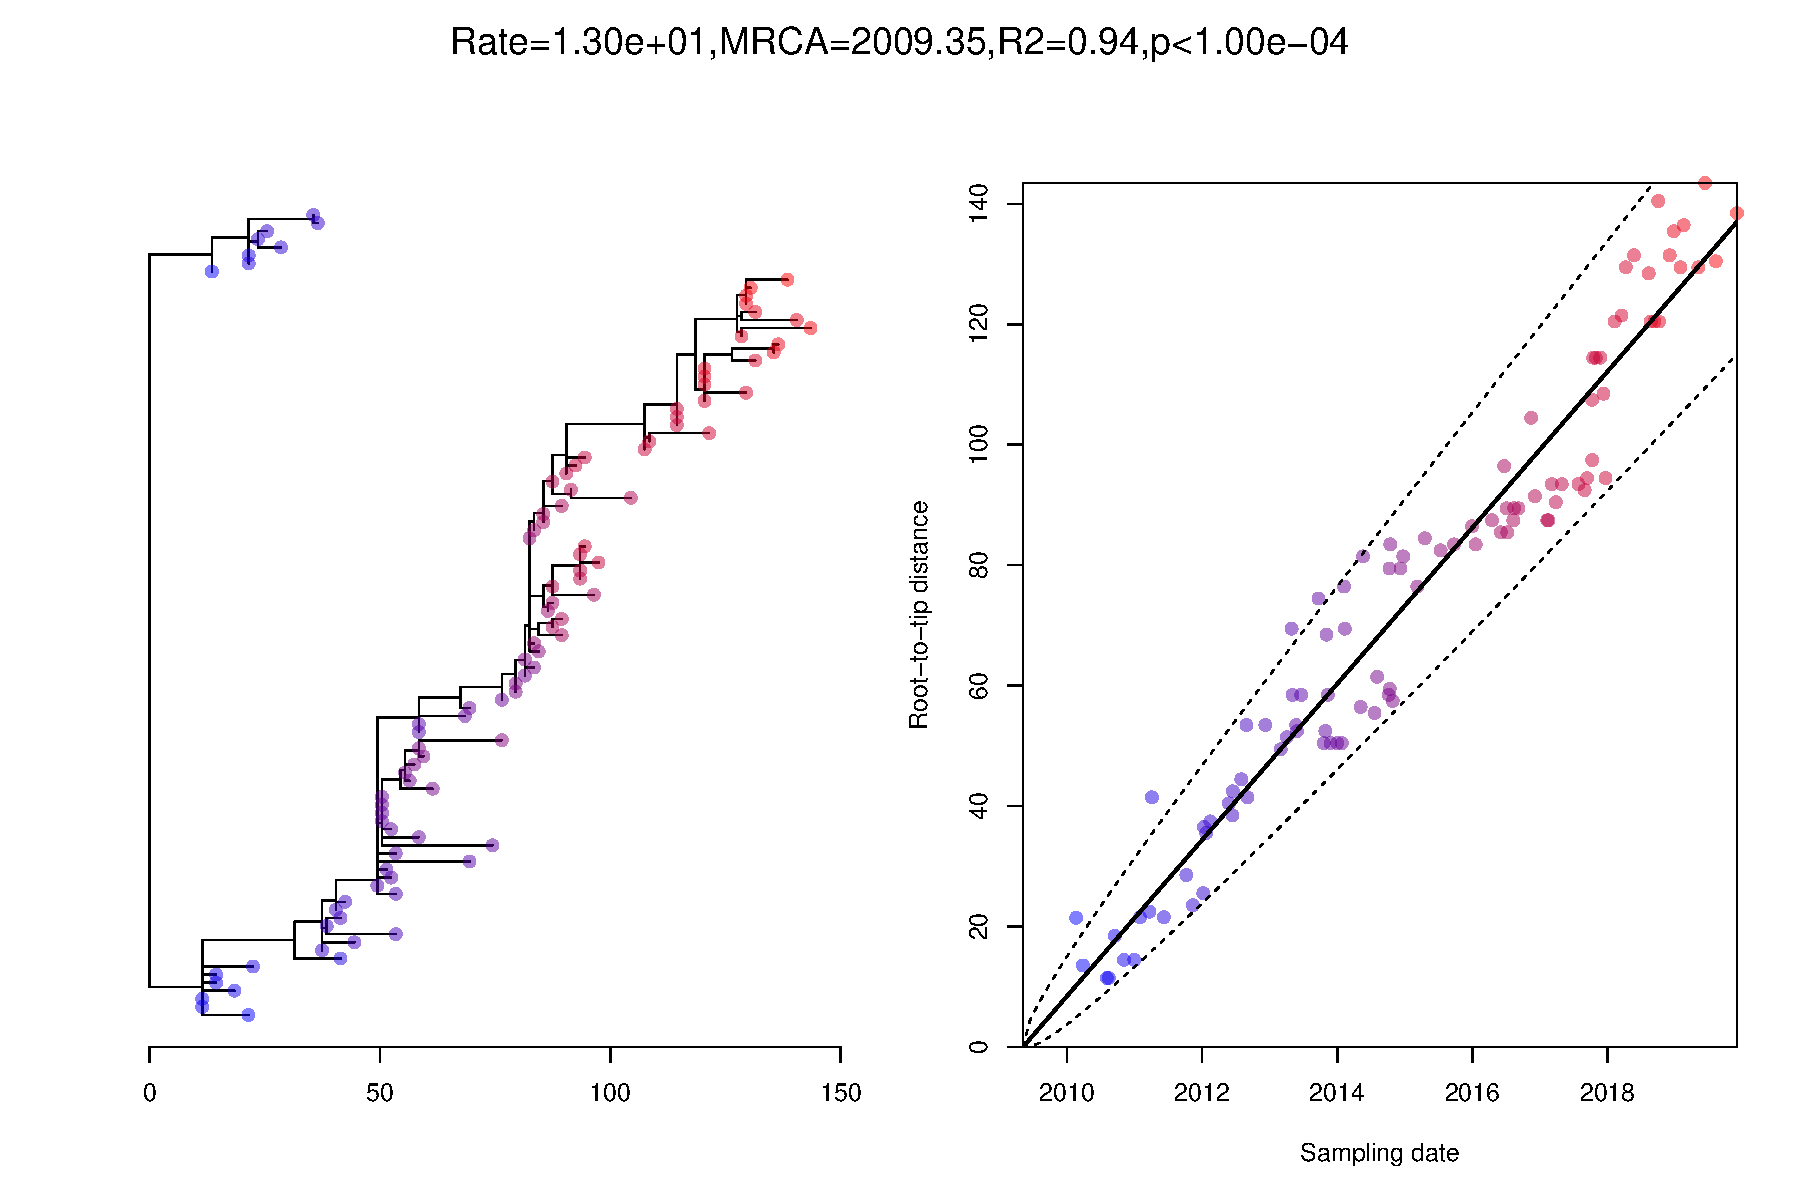
\includegraphics[width=15cm]{exampleS1.pdf}
\end{center}
\caption{Root-to-tip regression analysis for the motivating example.
\label{fig:exampleS1}}
\end{figure}

\begin{figure}[t!]
\begin{center}
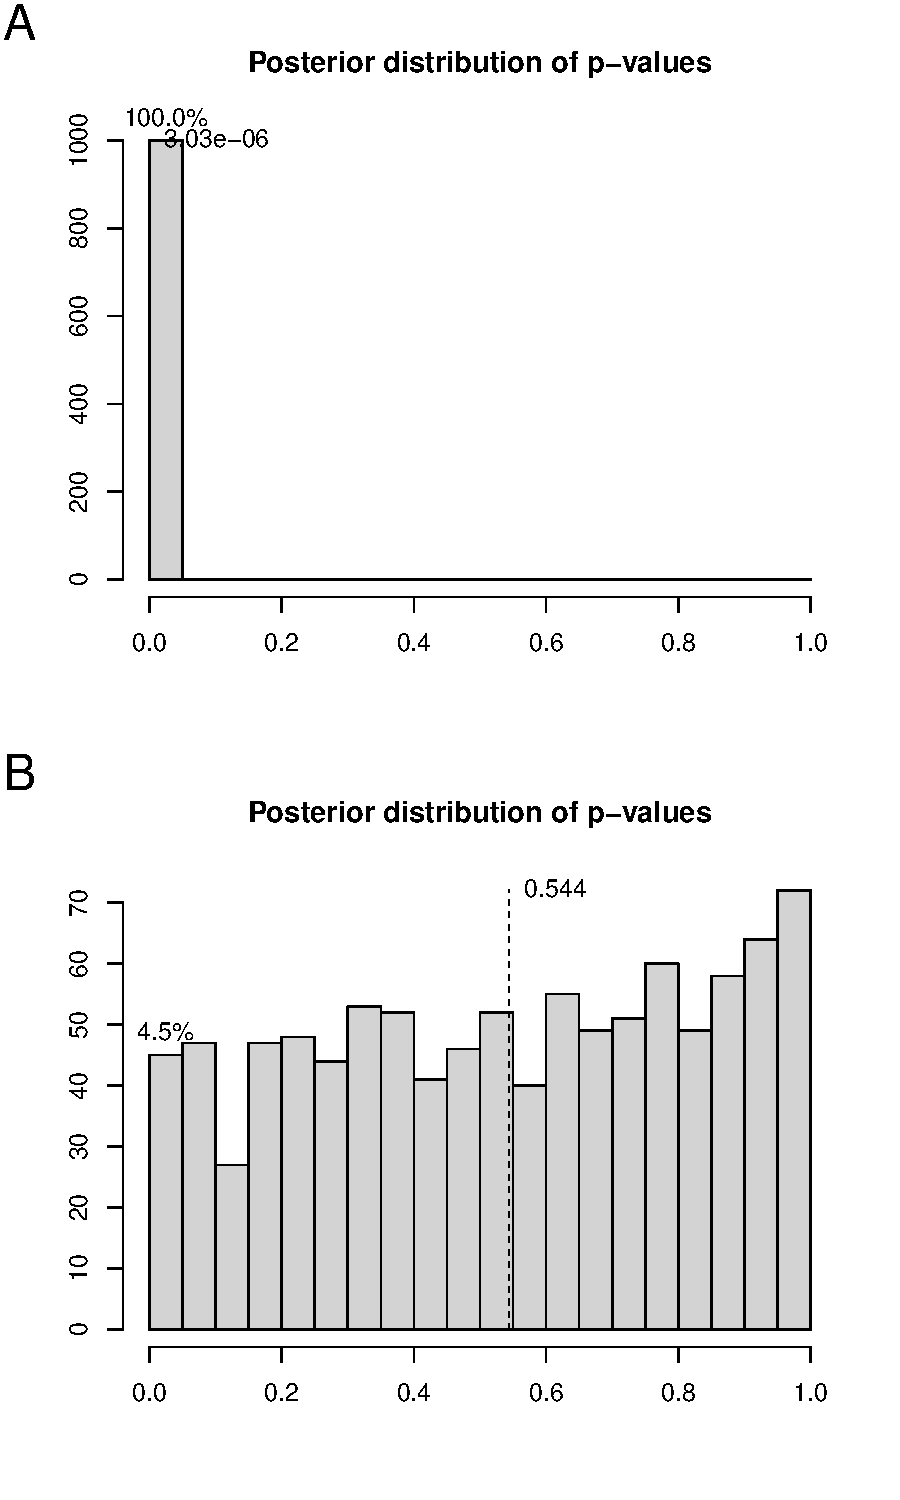
\includegraphics[width=15cm]{exampleS2.pdf}
\end{center}
\caption{Residuals after application on the motivating example of a strict clock model using LSD (A), node.dater (B), treedater (C) and TreeTime (D).
\label{fig:exampleS2}}
\end{figure}



\end{document}

%# Done so far
%
%- Dating via node.dating, BactDating, treedater, TreeTime and LSD2
%- Reproduce confounding effect described by Murray2016 on similar coalescent simulation, cf `confounding.Rmd`
%- Ruled out possible problem in phylogenetics since working directly with trees, not genetic data
%- Ruled out possible problem with root identification (ie consider root known)
%- Ruled out possible problem with multifurcation at the root (relaxed this in simulation)
%- More general version in `confounding-simstructure.Rmd` in which sampling dates do not have to be identical, and population sizes do not have to be constant. Simulation code is in `simStructure.R`, uses some of mlesky code for simulation of non-homogeneous Poisson coalescent process.
%- Difficult to get confusion using DetectImports simulations, cf `confounding-detectimports.Rmd`. May be because confusion only happens when sampling dates are biased, whereas DetectImports assumes sampling according to relative prevalence of populations
%- A Mendel test has been proposed to detect when confounding might happen, but this will flag an issue even if there is no structure and no problem with dating, cf `struture-test.Rmd`
%- When there is no confounding issue but the temporal signal is weak, eg because all sampling dates are the same or very similar, see `run-nosignal.Rmd`. Estimate incorrectly high clock rate. But the permutation test shows this is not to be trusted.
%

%Urgent TODO list
%Function for making a resDating object from a dated tree and a standard phylogeny which could be unrooted
%Use this eg in perfect residuals vignette and also the runDating subfunctions
%Also use in readme?
%Allow root inference
%Clock relaxation only works in BactDating currently
%Investigate false positives

%# Old to do
%
%- Propose new test to detect when the confounding problem happens
%- Implemented first naive idea of doing a Kruskal-Wallis test comparing the dates on the left and right for each node, cf testConfounding.R. Get false positive in structure-test.Rmd. Need better test, accounting for branch lengths. Maybe idea of using pseudo-residuals.
%- Propose a solution to when the confounding problem happens, maybe via removal of some leaves until test satisfied
%- Is permutation test useful?
%- Is clustered permutation test useful?
%- Comparison with run in which all leaves have same date. Attractive as only need to run once. Use DIC or something else?
%- Use better Bayesian model comparison methods?
%- Use Bayesian model criticism approach? Maybe using posterior predictive p-values?
%- Effect of relaxed clock models, especially ARC.
%- Effect of priors, especially on tree (constant effective population size as in Murray2016) but also others.
%- Apply to real data. May be able to reuse data from Holden2013, cf Fig S4 in Murray2016.
%
%# Some ideas
%
%- Fit with all dates equal using modified BactDating. Need to add move to scale up tree and down rate simultaneously, and vice versa. Consider prior effect. Given this fit, do posterior predictive test to see if there is a temporal signal. 
%- Joint model with and without temporal signal, to estimate Bayes Factor directly with rjMCMC. Current moves on sampling times could be starting point. 
%- Show confounding only happens when we have structure plus uneven sampling between structure component. Develop test for this based on undated phylgeny plus sampling dates. Bit like treeBreaker with continuous phenotype representing sampling dates.
%- Can a relaxed clock with high relaxation parameter equate a lack of temporal signal? What happens in ARC if omega is very high?
%- Alternate method to simulate confounding tree: generate very large phylogeny and subsample from large clusters within in
%- Shiny app
%- Consider sample of dated trees rather than point estimate

